% ==============================================================================
% 第 20 章：逐步求精 (Chapter 20: Iterative Refinement)
% ==============================================================================

\chapter{逐步求精}
\label{sec:ch20_refinement}

当你着手开发面向真实世界的程序时，往往需要面对极其复杂的信息形态，以及如何用程序数据来精确刻画这些信息的问题。应对这一挑战的最佳策略是采用\term{逐步求精}（iterative refinement）——这是科学探索中久经考验的方法论。

科学家的核心任务是使用某种数学形式来描述客观世界的一部分，这种努力的产物被称为\term{模型}（model）。随后，科学家通过各种方式测试模型，尤其是预测实验的结果。如果预测值与实际测量值之间的偏差过大，科学家就会精炼改进该模型，以提高预测的精度。这一迭代过程持续进行，直到预测足够准确为止。

考虑一位希望预测火箭飞行轨迹的物理学家：起初将“火箭视为质点”的模型固然简单，但也非常粗糙，因为它完全无法解释空气阻力。为此，物理学家随后加入了火箭的几何外形，并引入必要的空气动力学方程来计算阻力——这第二个模型就是对第一个模型的精炼。通过反复迭代，预测精度逐步收敛到令人满意的程度。

计算机科学专业的程序员也应当像这位物理学家一样工作。其核心在于找到现实世界信息的精准数据表示，并设计能够恰当处理这些数据的函数。复杂场景要求我们经历由简入繁的精炼过程，从最核心的信息要素出发，逐步添加细节。有时，在程序交付部署后，因用户提出新需求，程序员也必须对模型实施进一步的精炼。

到目前为止，我们在遇到复杂数据形态时已多次在幕后为你运用了逐步求精。本章将以一个综合性案例——计算机文件系统（目录树）的建模与处理——来系统演示作为程序开发核心原则的逐步求精。我们将探讨文件系统的本质，并逐步迭代构建出三个层层深入的数据表示。

\section{数据分析 }
\label{sec:20.1_data_analysis}

在关闭计算机或退出 DrRacket 之前，你必须确保你的所有工作都已安全保存，否则下次启动时就必须重头再来。因此，你让计算机将程序和数据存入\term{文件}（file）中。从抽象视角看，文件大体上可以看作是一段字符串（在底层则是连续的字节序列）。

在现代操作系统中，文件被组织在\term{目录}（directory，通常也称文件夹 folder）之中。简而言之，一个目录包含若干个文件以及若干个更深层的目录。后者被称为\term{子目录}（sub-directory），子目录内部又可以嵌套包含更多的子目录与文件。基于这种层次化结构，我们称之为\term{目录树}（directory tree）。

图~\ref{fig:123} 展示了一个小型的目录树示意图。与计算机科学中常见的“根节点在上”的画法不同，本图按照自然界树木的生长方向自底向上绘制：根目录名为 \code{TS}。根目录下包含一个名为 \code{read!} 的文件，以及名为 \code{Text} 和 \code{Libs} 的两个子目录。\code{Text} 目录下仅包含 3 个文件；而 \code{Libs} 目录下包含两个子目录，每个子目录下又包含各自的文件。每个方框右上角标明了类型属性：目录标记为 \code{DIR}，文件则标记为其大小（以整数表示所占字节或存储单位）。

\begin{figure}[htbp]
  \centering
  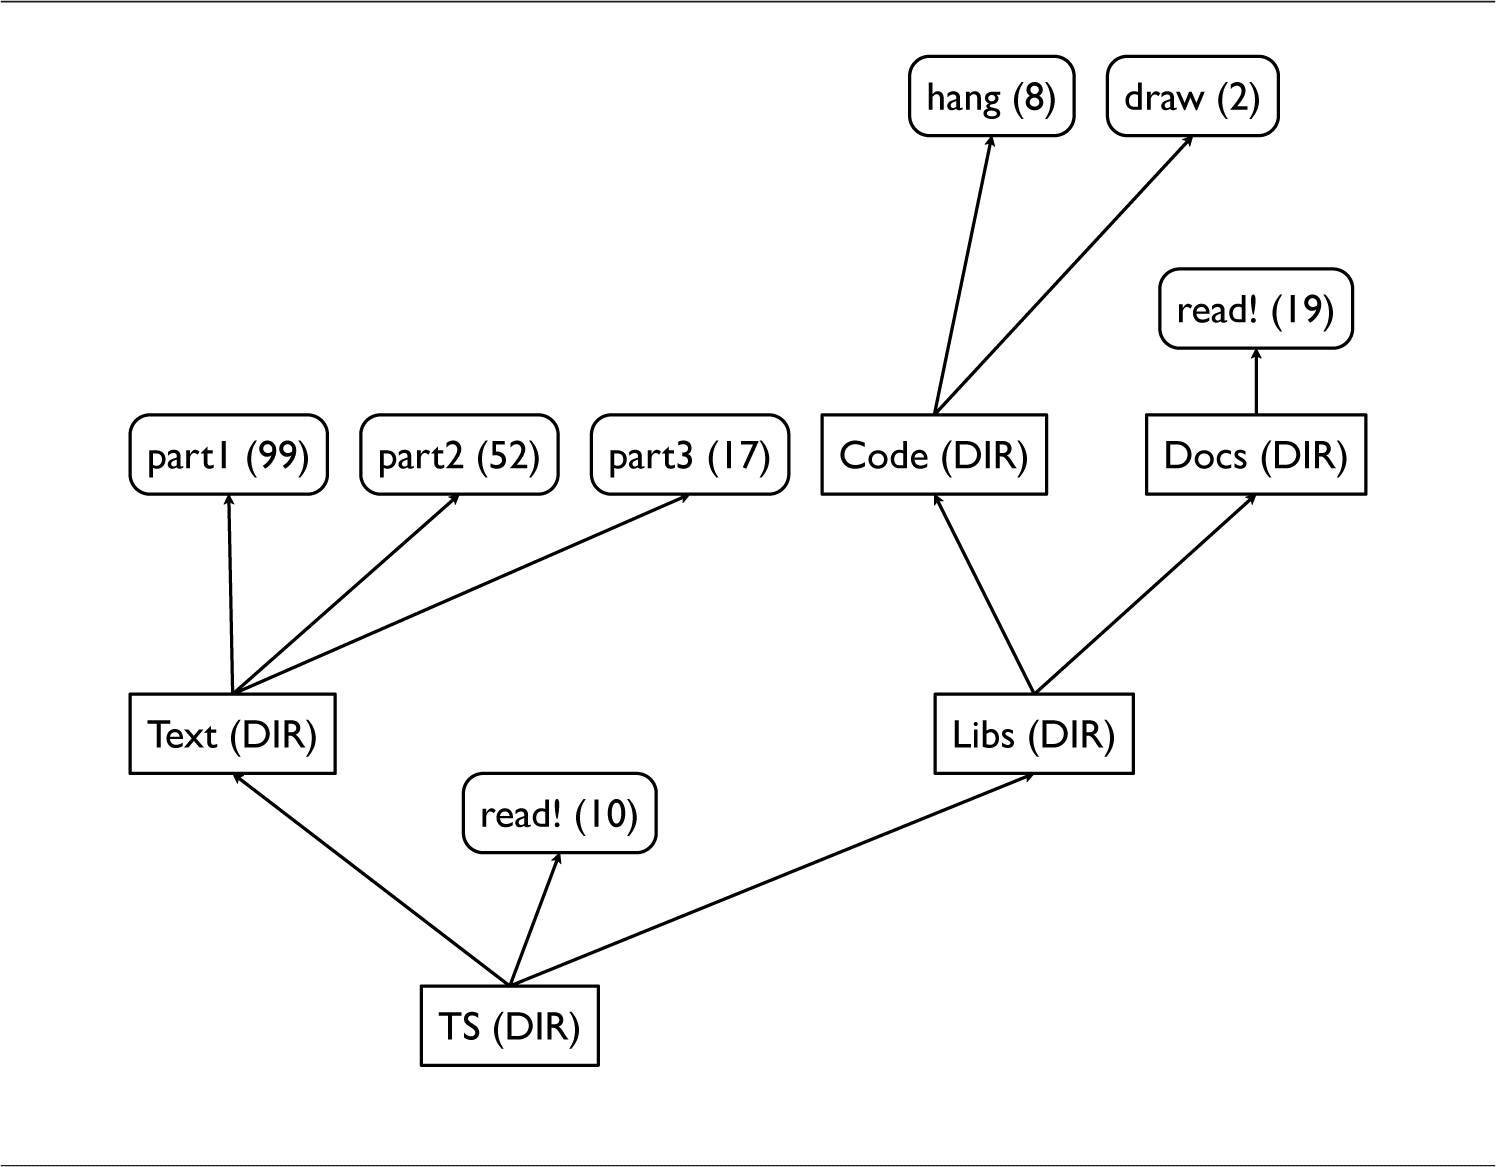
\includegraphics[width=0.85\textwidth]{images/00481.png}
  \caption{样本目录树 TS (A sample directory tree)}
  \label{fig:123}
\end{figure}

\begin{exercise}{分析样本目录树 TS}{329}
观察图~\ref{fig:123} 中的目录树 \code{TS}：
\begin{enumerate}
  \item 名为 \code{read!} 的文件在整棵树中共出现了多少次？你能写出从根目录到各次出现的完整路径吗？
  \item 该目录树中所有文件的总大小是多少？
  \item 若每个目录节点本身也占用 1 个单位的存储空间，整个目录树的总开销是多少？
  \item 该目录树共嵌套了多少层目录？
\end{enumerate}
\end{exercise}

\section{逐步细化数据定义}
\label{sec:20.2_refining_data}

练习 329 列举了用户对文件系统日常提出的典型查询。操作系统内核提供了各种命令来解答这些问题。为了设计类似的程序，我们必须建立目录树的数据表示。

我们在本节通过三次迭代，逐步提炼出三个数据模型。在每个阶段，我们权衡包含哪些属性，抽象忽略哪些细节。

\subsection{模型 1：文件为原子，目录为容器}

在最简视角下，用户将文件视为具有名字的原子实体，而将目录单纯视为容纳文件与其他目录的“容器”。基于此，我们将目录表示为列表，将文件表示为字符串（即文件名）：

\begin{lstlisting}[language=BSL]
; 一个 Dir.v1（目录版本 1）是下列之一：
; -- '()
; -- (cons File.v1 Dir.v1)
; -- (cons Dir.v1 Dir.v1)

; 一个 File.v1 是一个 String。
\end{lstlisting}

后缀 \code{.v1} 用于区分后续的精炼版本。

\begin{exercise}{将目录树表示为模型 1 数据}{330}
根据模型 1 的数据定义，将图~\ref{fig:123} 中的目录树 \code{TS} 翻译为 BSL 数据表示。
\end{exercise}

\begin{exercise}{统计模型 1 中的文件数}{331}
设计函数 \code{how-many}，统计给定 \code{Dir.v1} 中包含的文件总数。请严格遵循设计配方，并利用练习 330 的数据用例进行测试。
\end{exercise}

\subsection{模型 2：引入具名目录结构体}

模型 1 虽然简单，但抹杀了目录的重要本质——在模型 1 中，目录自身没有名字！我们无法列出某目录下所有子目录的名称。为了更忠实地反映现实，我们必须引入一个将“名称”与“内容容器”结合起来的结构体类型：

\begin{lstlisting}[language=BSL]
(define-struct dir [name content])

; 一个 Dir.v2 是一个结构体：
;   (make-dir String LOFD)

; 一个 LOFD（List-of-Files-and-Directories，文件与目录列表）是下列之一：
; -- '()
; -- (cons File.v2 LOFD)
; -- (cons Dir.v2 LOFD)

; 一个 File.v2 是一个 String。
\end{lstlisting}

请注意：\code{Dir.v2} 引用了 \code{LOFD}，而 \code{LOFD} 又回引了 \code{Dir.v2}。这是一对\textbf{相互递归}的数据定义。

\begin{exercise}{将目录树表示为模型 2 数据}{332}
根据模型 2 的数据定义，将图~\ref{fig:123} 中的目录树 \code{TS} 翻译为数据表示。
\end{exercise}

\begin{exercise}{统计模型 2 中的文件数}{333}
设计函数 \code{how-many}，统计给定 \code{Dir.v2} 中包含的文件总数。将你的函数实现与练习 331 进行对比。
\end{exercise}

\begin{exercise}{扩展目录属性：大小与可读性}{334}
展示如何为目录结构体增加两个属性：大小（size，衡量目录元数据自身所占的空间）与可读性（readability，指定除所有者外的其他人是否可以浏览该目录内容）。给出相应的结构体定义与数据定义。
\end{exercise}

\subsection{模型 3：文件属性与子项拆分}

现实中的文件不仅有文件名，还包含文件大小、修改日期与内容。我们为文件定义专用的结构体：

\begin{lstlisting}[language=BSL]
(define-struct file [name size content])

; 一个 File.v3 是一个结构体：
;   (make-file String N String)
\end{lstlisting}

同时，在目录结构体中，将“文件列表”与“子目录列表”清晰地分开存放，不仅逻辑更分明，处理起来也更加模块化：

\begin{lstlisting}[language=BSL]
(define-struct dir.v3 [name dirs files])

; 一个 Dir.v3 是一个结构体：
;   (make-dir.v3 String Dir* File*)

; 一个 Dir* 是下列之一：
; -- '()
; -- (cons Dir.v3 Dir*)

; 一个 File* 是下列之一：
; -- '()
; -- (cons File.v3 File*)
\end{lstlisting}

按照计算机科学传统，名称末尾加 \code{*}（星号）表示“多个”，以区分单数实体 \code{Dir.v3} 与复数集合 \code{Dir*}。

\begin{exercise}{将目录树表示为模型 3 数据}{335}
按照模型 3 的数据定义，将图~\ref{fig:123} 中的目录树 \code{TS} 转换为数据表示，文件内容统一使用空字符串 \code{""}。
\end{exercise}

\begin{exercise}{统计模型 3 中的文件数}{336}
设计函数 \code{how-many}，统计给定 \code{Dir.v3} 中包含的文件总数。面对高度复杂的相互递归数据定义，你为什么能够坚信自己的函数计算结果是完全正确的？
\end{exercise}

\begin{exercise}{使用 List-of 抽象与高阶函数重构}{337}
利用 \code{List-of} 抽象重新定义 \code{Dir.v3}：
\begin{lstlisting}[language=BSL]
(define-struct dir.v3 [name dirs files])
; 一个 Dir.v3 是：(make-dir.v3 String [List-of Dir.v3] [List-of File.v3])
\end{lstlisting}
随后利用 ISL+ 中的列表高阶处理函数（如 \code{foldr}、\code{map}），重新实现练习 336 中的 \code{how-many}。
\end{exercise}

\section{逐步细化函数}
\label{sec:20.3_refining_functions}

为了使后续练习更具实战感，DrRacket 提供了 \code{htdp/dir} 教学库。该库内置了模型 3 的结构体定义（去掉了 \code{.v3} 后缀），并提供了一个能够直接读取你电脑真实目录树的函数：

\begin{lstlisting}[language=BSL]
(require htdp/dir)

; String -> Dir
; 读取路径 a-path 所指的真实目录，生成对应的 Dir 数据表示
(define (create-dir a-path) ...)
\end{lstlisting}

例如，在定义区输入并运行：
\begin{lstlisting}[language=BSL]
(define O (create-dir "/Users/matthias/")) ; OS X
(define L (create-dir "/var/log/"))        ; Linux
(define W (create-dir "C:\\Users\\..."))    ; Windows
\end{lstlisting}
你就能获得本地磁盘的真实目录数据结构！

\begin{notebox}[使用注意]
1. 对于非常庞大的目录树，DrRacket 构建数据表示可能需要较长时间。请首先在小型文件夹上试验。\\
2. \textbf{不要}在代码中自行用 \code{define-struct} 定义 \code{dir} 和 \code{file}，因为引入教学包后二次定义会导致命名冲突。
\end{notebox}

在后续练习中，路径（Path）被表示为由目录和文件名构成的字符串列表：
\begin{lstlisting}[language=BSL]
; 一个 Path 是一个 [List-of String]
; 解释：指引进入目录树深处的路径导航序列
\end{lstlisting}
例如在图~\ref{fig:123} 中，从根目录 \code{TS} 到 \code{part1} 的路径为 \code{(list "TS" "Text" "part1")}。

\begin{exercise}{在真实文件系统上运行 how-many}{338}
利用 \code{create-dir} 将你电脑上的某个目录转化为数据表示，然后调用练习 336 中的 \code{how-many} 统计其文件数。借助系统自带的文件管理器验证其准确性。
\end{exercise}

\begin{exercise}{搜索指定文件是否存在 find?}{339}
设计函数 \code{find?}。该函数接收一个 \code{Dir} 与一个文件名，判断该目录树中是否存在具有该名称的文件。
\end{exercise}

\begin{exercise}{列出所有文件与目录名 ls}{340}
设计函数 \code{ls}，列出给定 \code{Dir} 及其所有嵌套子目录中包含的所有文件和目录的名字列表。
\end{exercise}

\begin{exercise}{计算目录总占用空间 du}{341}
设计函数 \code{du}，接收一个 \code{Dir} 并计算其整棵目录树占用的总存储空间。假设存储每个目录节点本身固定消耗 1 个单位空间。
\end{exercise}

\begin{exercise}{查找文件的完整路径 find}{342}
设计函数 \code{find}。该函数接收目录 \code{d} 与文件名 \code{f}。若该文件存在，返回通往该文件的路径；若不存在，返回 \code{\#false}。

\emph{进阶挑战：} 图~\ref{fig:123} 中有两个名为 \code{read!} 的文件，基本的 \code{find} 通常只能返回其中一条路径。设计函数 \code{find-all}，返回所有能够找到 \code{f} 的路径列表。
\end{exercise}

\begin{exercise}{递归列出所有文件的完整路径 ls-R}{343}
设计函数 \code{ls-R}，列出给定目录树中所有文件的完整路径列表。
\end{exercise}

\begin{exercise}{组合式设计重构 find-all}{344}
使用练习 343 中的 \code{ls-R} 重新设计练习 342 中的 \code{find-all}。这就是通过函数组合（design by composition）解决复杂问题的高阶范式。
\end{exercise}
